\section{Результаты работы 7 лабораторной работы}

\subsection{Аналитический раздел}

Цель: продолжение знакомства с существующими методиками предварительной оценки параметров программного проекта и практическая оценка затрат по модели COCOMO II.

Метод функциональных точек
В этом методе рассматривается не размер, а функциональность или полезность продукта, в качестве количественной характеристики применяется понятие количества функциональных точек. 

Количество функциональных точек – количественная характеристика, обозначается как FP (function points).

Функциональная точка — единица измерения функциональности ПО. Функциональность программы связана с обработкой информации по запросу пользователя и не зависит от применяемых технических решений. 

Пользователи — отправители и целевые получатели данных (люди, смежные интегрированные информационные системы).

Оценка трудозатрат может быть выполнена на ранних стадиях работы над проектом, поскольку в основе лежит изучение требований.

Функциональность системы определяется:

функциональными типами

элементарными процессами

Типы элементарных процессов, используемых в методе функциональных точек:

внешний ввод (EI) — элементарный процесс, перемещающий данные из внешней среды в приложение;

внешний вывод (ЕО) — элементарный процесс, перемещающий данные, вычисленные в приложении, во внешнюю среду;

внешний запрос (EQ) — элементарный процесс, состоящий из комбинации «запрос/ответ», не связанный с вычислением производных данных;

внутренний логический файл (ILF) — выделяемые пользователем логически связанные группы данных, которые поддерживаются внутри продукта и обслуживается через внешние вводы;

внешний интерфейсный файл (EIF) — выделяемые пользователем логически связанные группы данных или блоки управляющей информации, на которые ссылается продукт, но которые поддерживаются вне продукта.

\subsubsection{Задание}

Компания получила заказ на разработку клиентского мобильного приложения брокерской системы. Программа позволяет просматривать актуальную биржевую информацию, производить сделки и отслеживать их выполнение.
Приложение имеет 4 страницы: авторизация, биржевые сводки, заявки, новая заявка.

\textbf{Характеристики команды, продукта и проекта}

Разработанное ПО состоит из трех компонентов. Первый компонент составляет по объему примерно 15% программного кода и будет написан на SQL, второй (около 60% кода) - на С#, а третий в объеме 25% кода - на Java. 

Характеристики продукта: 

\begin{enumerate}
	\item Обмен данными - 5. 
	\item Распределенная обработка -5
	\item Производительность -3
	\item Эксплуатационные ограничения по аппаратным ресурсам – 2 
	\item Транзакционная нагрузка – 3
	\item Интенсивность взаимодействия с пользователем (оперативный ввод данных) – 4
	\item Эргономические характеристики, влияющие на эффективность работы конечных пользователей – 1
	\item Оперативное обновление – 4
	\item Сложность обработки – 4
	\item Повторное использование – 0
	\item Легкость инсталляции – 1
	\item Легкость эксплуатации/администрирования – 2
	\item Портируемость – 2
	\item Гибкость – 2.
\end{enumerate}

Для реализации проекта была сформирована новая команда разработчиков, у отдельных членов которой имеется некоторый опыт создания систем подобного типа. В целях сплочения команды были проведены определенные мероприятия, что обеспечило на старте проекта приемлемую коммуникацию внутри коллектива. Заказчик не настаивает на жесткой регламентации процесса, однако график реализации проекта довольно жесткий. Несмотря на то, что предметная область является для разработчиков относительно новой, анализу архитектурных рисков было уделено лишь некоторое внимание. Организация только начинает внедрять методы управления проектами и формальные методы оценки качества процесса разработки. 

Надежность и уровень сложности (RCPX) разрабатываемой системы оцениваются как очень высокие, повторного использования компонентов не предусматривается (RUSE). Возможности персонала (PERS) – средние, его опыт работы в разработке систем подобного типа (PREX) низкий. Сложность платформы (PDIF) высокая. Разработка предусматривает очень интенсивное использование инструментальных средств поддержки (FCIL). Заказчик настаивает на жестком графике (SCED).

\subsubsection{Авторизация}

На данной странице осуществляется ввод логина и пароля пользователя для входа в систему. Страница содержит два поля ввода и одну командную кнопку, а также флажок-переключатель, который активируется при необходимости запоминания параметров авторизации.

\begin{figure}[ht!]
	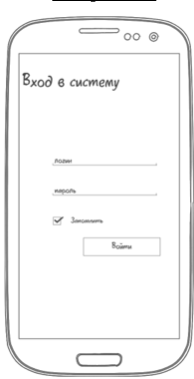
\includegraphics[width=0.3\linewidth]{assets/images/1.1 Авторизация.png}
	\label{fig:r2}
	\caption{Авторизация}
\end{figure}
\FloatBarrier

\textbf{Внутренний логический файл (ILF)}

1 соответствующая таблица в базе данных, поля «Логин», «Пароль» и 1 локальный файл

\begin{itemize}
	\item Таблица в базе данных: Количество типов элементарных записей (RET) = 1 и логин, и пароль представляются в формате строки.
	\item Количество типов элементарных данных (DET) = 2 (логин, пароль).
	\item Локальный файл
	\item Количество типов элементарных записей (RET) = 1 и логин, и пароль представляются в формате строки.
	\item Количество типов элементарных данных (DET) = 2 (логин, пароль).
\end{itemize}



\textbf{Внешний ввод (EI)}

\begin{itemize}
	\item запоминание данных пользователя
	\item FTR = 2 (2 файла)
	\item DET = 4 (поля логин, пароль, флажок-переключатель «Запомнить», кнопка «Войти»)

\end{itemize}

\textbf{Внешние запросы (EQ)}

\begin{itemize}
	\item запрос на авторизацию
	\item FTR = 1 (на логический файл)
	\item DET = 4 (поля логин, пароль, флажок-переключатель «Запомнить», кнопка «Войти»)
\end{itemize}


\subsubsection{Биржевые сводки}

Биржевые сводки отражают текущую ситуацию на бирже. Страница содержит таблицу, кнопку «Добавить» и диалоговое окно с одним полем для ввода и двумя командными кнопками (Ok, Cancel).


\begin{figure}[ht!]
	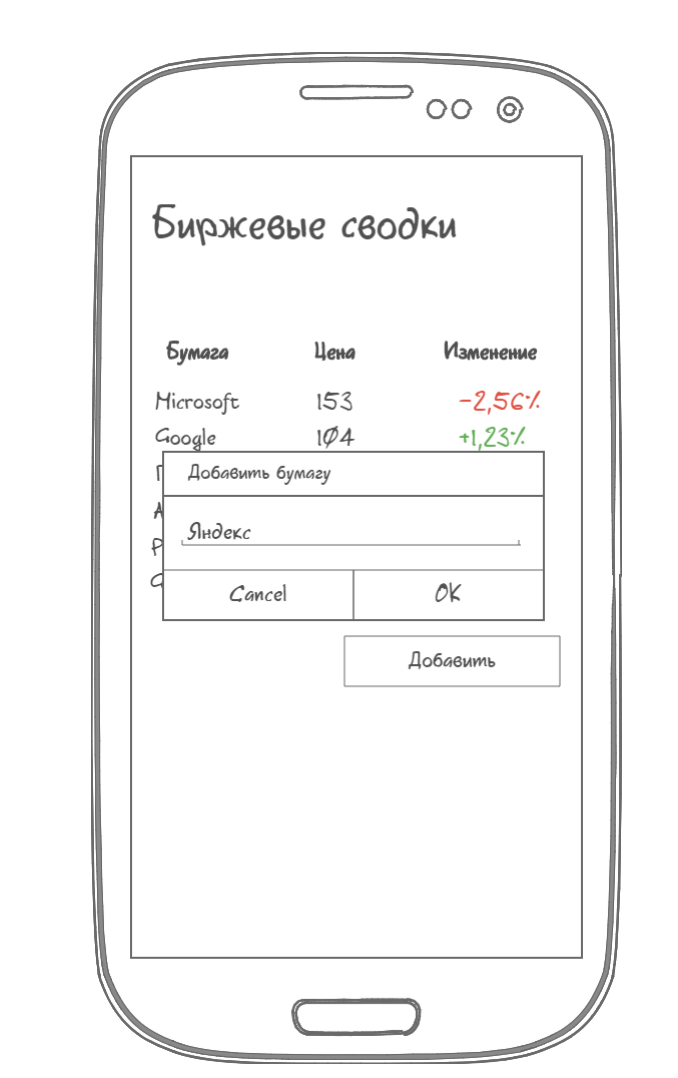
\includegraphics[width=0.3\linewidth]{assets/images/1.2 Биржевые сводики.png}
	\label{fig:r2}
	\caption{Биржевые сводики}
\end{figure}
\FloatBarrier

\textbf{Внутренний логический файл (ILF)}

1 соответствующая таблица в базе данных, поля «Ценная бумага», «Цена» (за одну ценную бумагу), «Изменение» (изменение цены бумаги со времени последнего закрытия биржи).

Количество типов элементарных записей (RET) = 2

\begin{itemize}
	\item «Ценная бумага» представляется в формате строки
	\item «Цена» и «Изменение» в вещественном формате.
\end{itemize}



Количество типов элементарных данных (DET) = 3 («Ценная бумага», «Цена», «Изменение»).

\textbf{Внешний ввод (EI)}

Добавить новую бумагу

FTR = 1 (запрос к таблице)

DET = 3 (кнопка «Добавить», поле названия, кнопка «Ok»)

\textbf{Внешний вывод (EO)}

Вывод информации о ценных бумагах

FTR = 2 (запрос к таблице и внешний интерфейсный файл)

DET = 3 (поля «Бумага», «Цена», «Изменение»)


\subsubsection{Завки}

Заявки содержат таблицу, отображающую текущие (еще не выполненные) заявки на покупку или продажу ценных бумаг. 
При нажатии на любую строку таблицы появляется контекстное меню с возможностью удалить или изменить заявку.

\begin{figure}[ht!]
	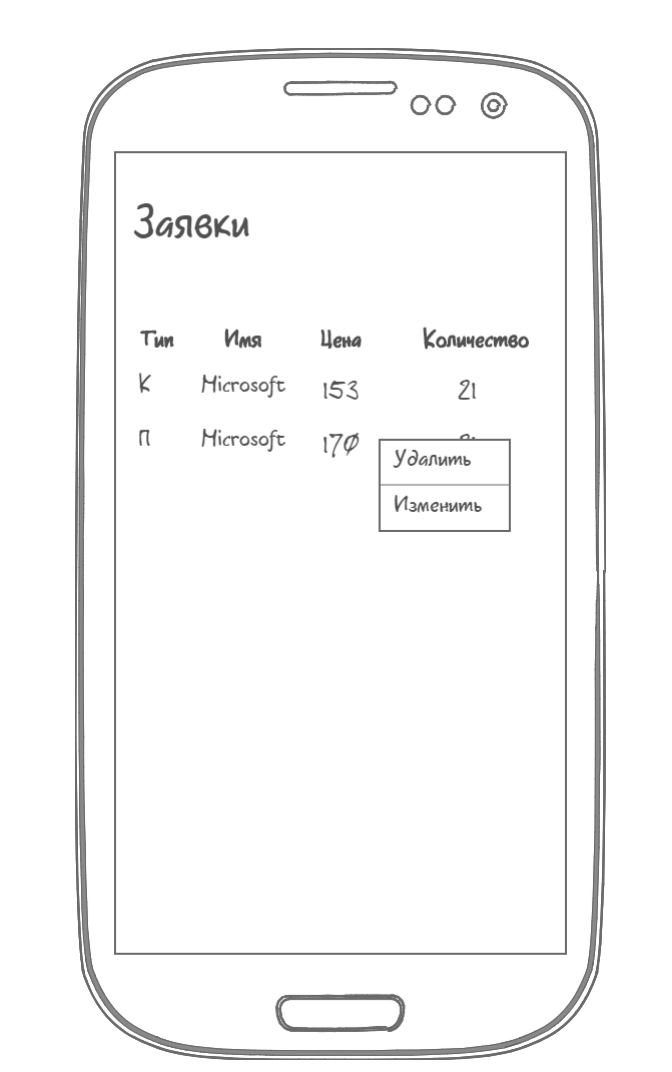
\includegraphics[width=0.3\linewidth]{assets/images/1.3 Заявка.png}
	\label{fig:r2}
	\caption{Заявки}
\end{figure}
\FloatBarrier

\textbf{Внутренний логический файл (ILF)}

1 соответствующая таблица в базе данных, поля «Тип» (покупка или продажа), «Имя», «Цена», «Количество».

Количество типов элементарных записей (RET) = 4

\begin{itemize}
	\item «Тип» представляется логическим типом, 
	\item «Имя» - строковый формат, 
	\item «Цена» - вещественный, 
	\item «Количество» - положительное целое число.
\end{itemize}

Количество типов элементарных данных (DET) = 4 («Тип», «Имя», «Цена», «Количество»).

\textbf{Внешний ввод (EI)}

Изменить заявку

FTR = 1 (запрос к таблице)

DET = 5 (строка из таблицы (поля «Тип», «Имя», «Цена», «Количество»), кнопка «Изменить»)

Удалить заявку

FTR = 1 (запрос к таблице)

DET = 5 (строка из таблицы (поля «Тип», «Имя», «Цена», «Количество»), кнопка «Удалить»)

\textbf{Внешний вывод (EO)}

Вывод информации о заявках

FTR = 1 (запрос к таблице)

DET = 4 (поля «Тип», «Имя», «Цена», «Количество»)

\subsubsection{Новая заявка}

Страница позволяет оформить заявку на покупку или продажу ценной бумаги.

\begin{figure}[ht!]
	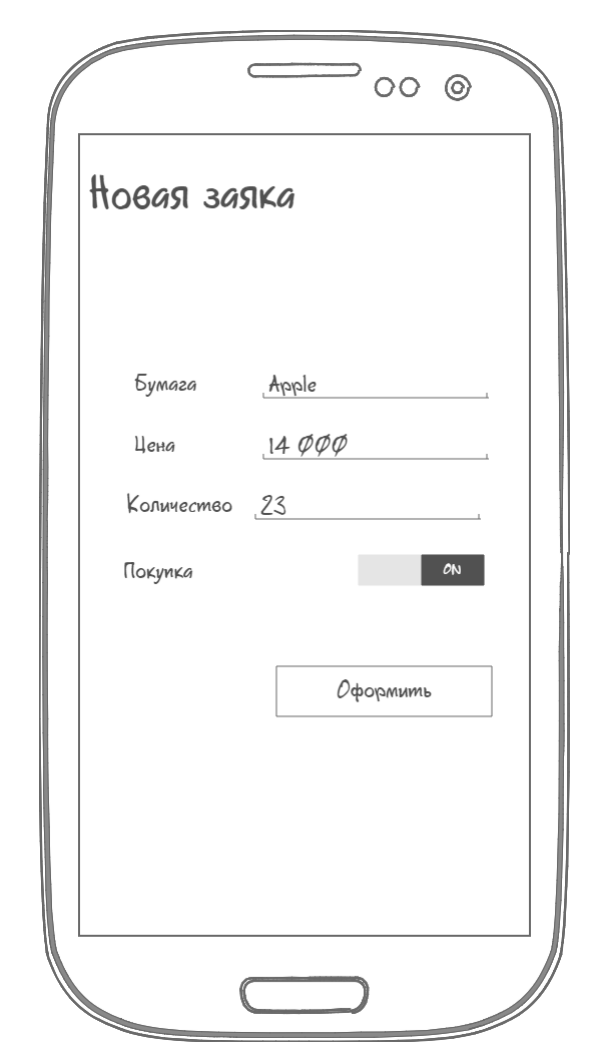
\includegraphics[width=0.3\linewidth]{assets/images/1.4 Заявки.png}
	\label{fig:r2}
	\caption{Заявки}
\end{figure}
\FloatBarrier

\textbf{Внутренний логический файл (ILF)}

1 соответствующая таблица в базе данных, поля «Бумага» (имя бумаги), «Цена», «Покупка» (булевая переменная в значении true – покупка, false - продажа).
Используется та же таблица, что и для страницы «Заявки», но используется только 3 поля: «Тип», «Имя», «Цена».

\textbf{Внешний ввод (EI)}

Продать/купить ценную бумагу

FTR = 1 (запрос к таблице)

DET = 5 (поля «Бумага», «Цена», «Количество», флаг «Покупка», кнопка «Оформить»)

\textbf{Внешний интерфейсный файл (EIF)}

RET = 2 (строка, вещественное число)

DET = 3 (3 таблицы)

Итого:

\begin{enumerate}
	\item уровень сложности логического файла – низкий;
	\item уровень сложности внешних выводов – низкий;
	\item уровень сложности внешних вводов – низкий;
	\item уровень внешних запросов – низкий;
	\item уровень сложности внешних интерфейсных файлов – низкий.
\end{enumerate}

\begin{figure}[ht!]
	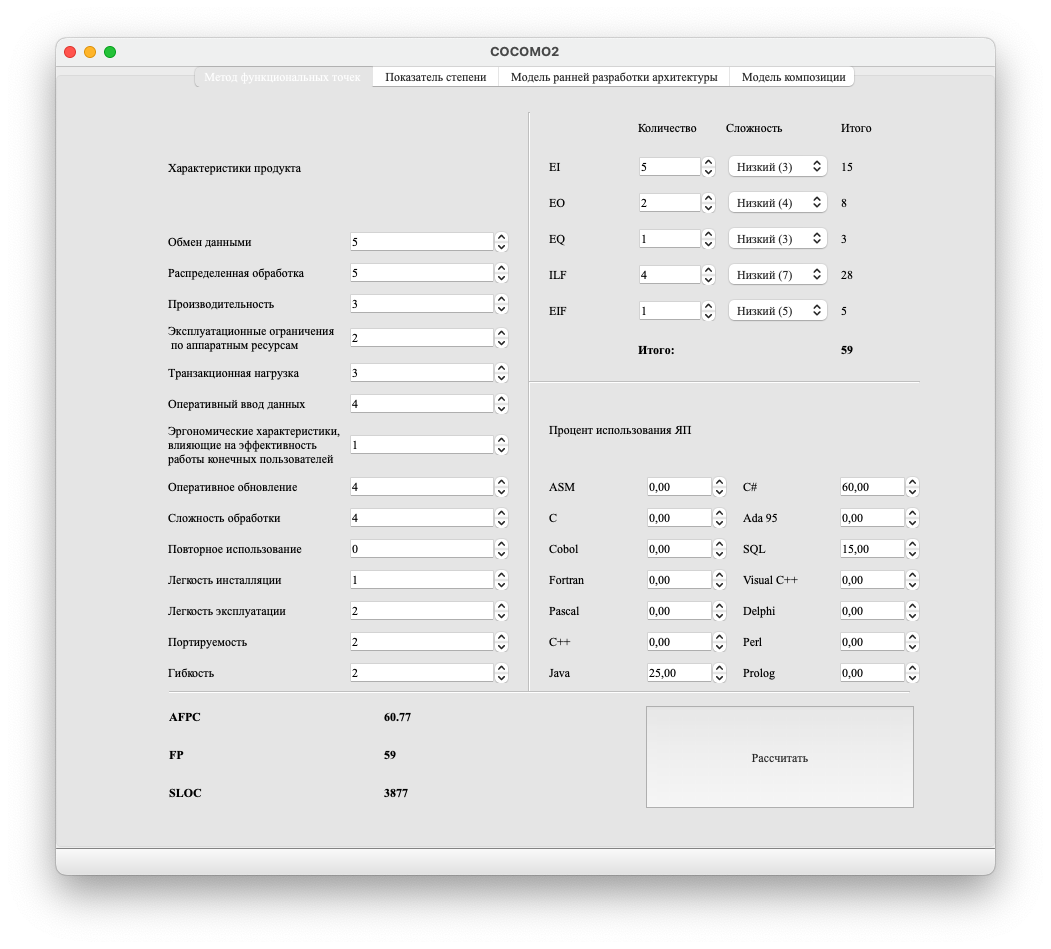
\includegraphics[width=1\linewidth]{assets/images/2.1.png}
	\label{fig:r2}
	\caption{Метод фукнциональных точек}
\end{figure}
\FloatBarrier

Нормированное количество функциональных точек: 60.77

Количество функциональных точек: 59

Количество строк исходного кода: 3877

\subsection{Методика COCOMO II}

3 модели оценки стоимости в COCOMO II:

\begin{enumerate}
	\item Модель композиции приложения – модель, которая подходит для проектов, созданных с помощью современных инструментальных средств. Единицей измерения служит объектная точка (учитывается количество экранов, отчетов и компонентов).
	
	\begin{itemize}
		\item рассматривается макетирование пользовательский интерфейсов
		\item  оценивается производительность
		\item определяется степень зрелости технологии
	\end{itemize}
	
	\item Модель ранней разработки архитектуры – модель применяется для получения приблизительных оценок проектных затрат периода выполнения проекта перед тем как будет определена архитектура в целом. В качестве единиц измерения используются функциональные точки либо KSLOC.
	\item Постархитектурная модель – наиболее детализированная модель СОСОМО II, которая используется после разработки архитектуры проекта. В состав этой модели включены новые драйверы затрат, новые правила подсчета строк кода, а также новые уравнения
\end{enumerate}

\begin{figure}[ht!]
	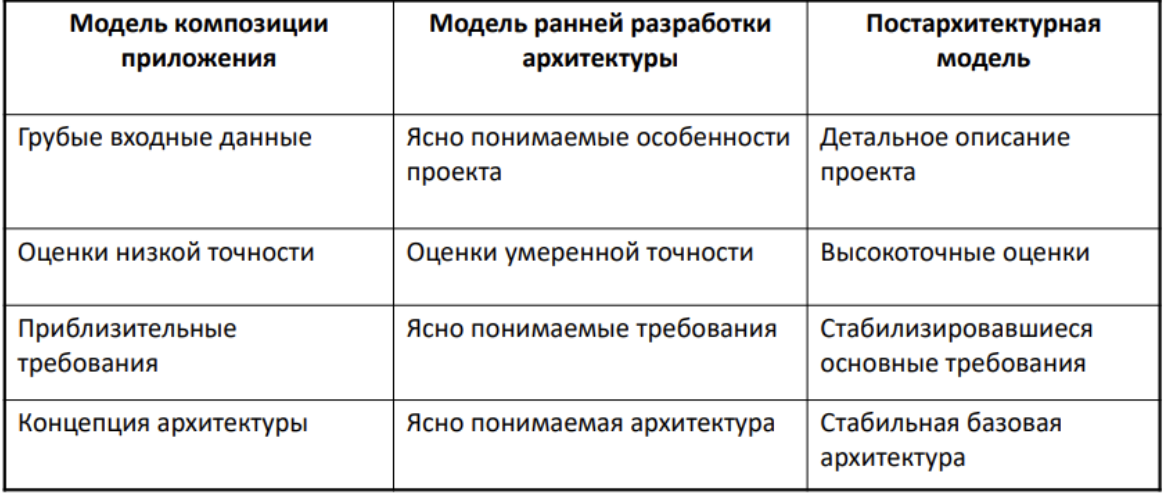
\includegraphics[width=1\linewidth]{assets/images/3.1 Table.png}
	\label{fig:r2}
\end{figure}
\FloatBarrier


Преимущества COCOMO2:

\begin{enumerate}
	\item возможен учет многих факторов;
	\item универсальный метод;
	\item фактические данные подбираются в соответствии с реальными проектами;
	\item метод позволяет добавлять уникальные факторы для корректировки характеристик;
	\item результаты прогнозирования сопровождаются обязательной документацией;
	\item модель проста в освоении и применении
\end{enumerate}

Недостатки COCOMO2:

\begin{enumerate}
	\item все результаты зависят от размера программного продукта;
	\item игнорируются требования к характеристикам качества программного продукта;
	\item игнорируется изменяемость требований к программному продукту;
	\item игнорируются многие особенности, связанные с аппаратным обеспечением проекта;
\end{enumerate}

Показатели проекта:

\begin{itemize}
	\item Новизна проекта (PREC) – полное отсутствие прецедентов, полностью непредсказуемый проект (т.к. была сформирована новая команда разработчиков, только отдельные члены имели некоторый опыт создания систем подобного типа)
	\item Гибкость процесса разработки (FLEX) – большей часть согласованный процесс (график жесткий, точной регламентации нет)
	\item Разрешение рисков в архитектуре системы (RESL) – некоторое (40 \%)
	\item Сплоченность команды (TEAM) – некоторая согласованность (команд новая, но были проведены определенные мероприятия по сплочению)
	\item Уровень развития процесса разработки (PMAT) – начальный уровень (только начинают внедрять)
\end{itemize}

Результат расчёта показателя степени P


\begin{figure}[ht!]
	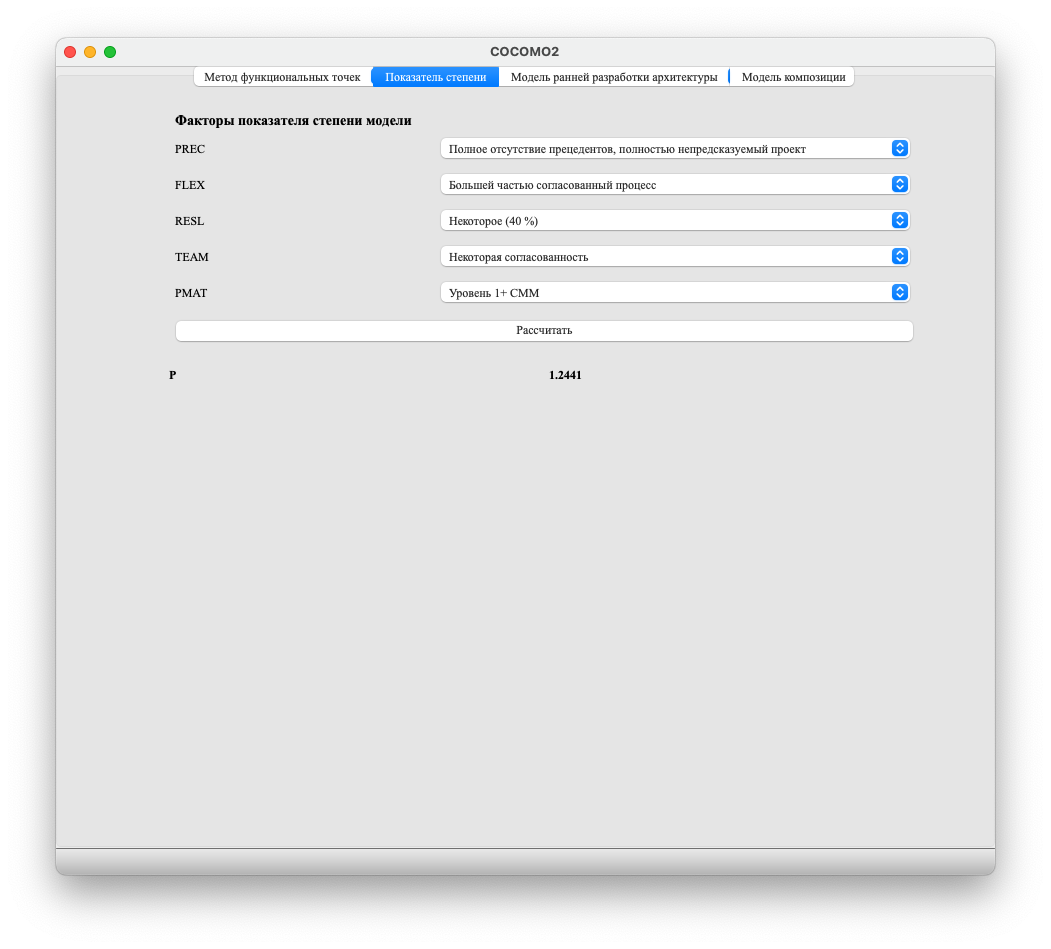
\includegraphics[width=1\linewidth]{assets/images/2.2.png}
	\label{fig:r2}
	\caption{Показатель степени}
\end{figure}
\FloatBarrier

(Средняя ЗП принята равной 60 000)

Расчёт модели композиции проекта. По страницам:

\begin{itemize}
	\item Авторизация – 3 простых поля и 1 средней сложности, 3 поколение
	\item Биржевые сводки – 3 простых поля и 1 средней сложности, 3 поколение
	\item Заявки - 1 простое поля и 2 средней сложности
	\item Новая заявка - 4 простых поля и 1 средней сложности
\end{itemize}

Итого:
\begin{itemize}
	\item Полей простой сложности: 11
	\item Полей средней сложности: 5
	\item Полей высокой сложности: 0
	\item Модулей на ЯП 3го поколения: 2
	\item Повторное использование: не предусматривается
	\item Опытность команды: низкая
\end{itemize}

\begin{figure}[ht!]
	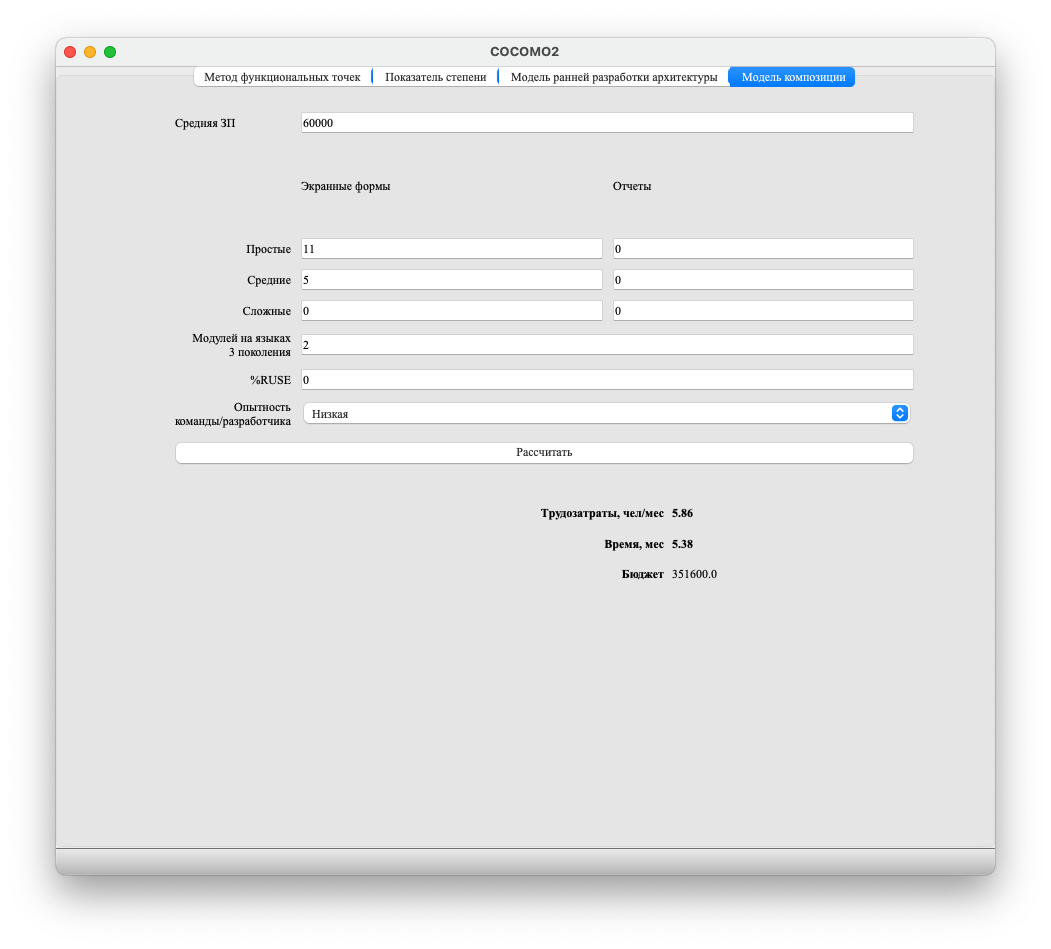
\includegraphics[width=1\linewidth]{assets/images/2.4.png}
	\label{fig:r2}
	\caption{Метод композиции}
\end{figure}
\FloatBarrier

Расчёт модели ранней разработки архитектуры:
\begin{itemize}
	\item Надежность и уровень сложности (RCPX) – очень высокие
	\item Повторное использования компонентов не предусматривается (RUSE). 
	\item Возможности персонала (PERS) – средние
	\item Опыт работы в разработке систем подобного типа (PREX) – низкий. 
	\item Сложность платформы (PDIF) – высокая. 
	\item Очень интенсивное использование инструментальных средств поддержки (FCIL). 
	\item Жесткий график (SCED)
\end{itemize}


\begin{figure}[ht!]
	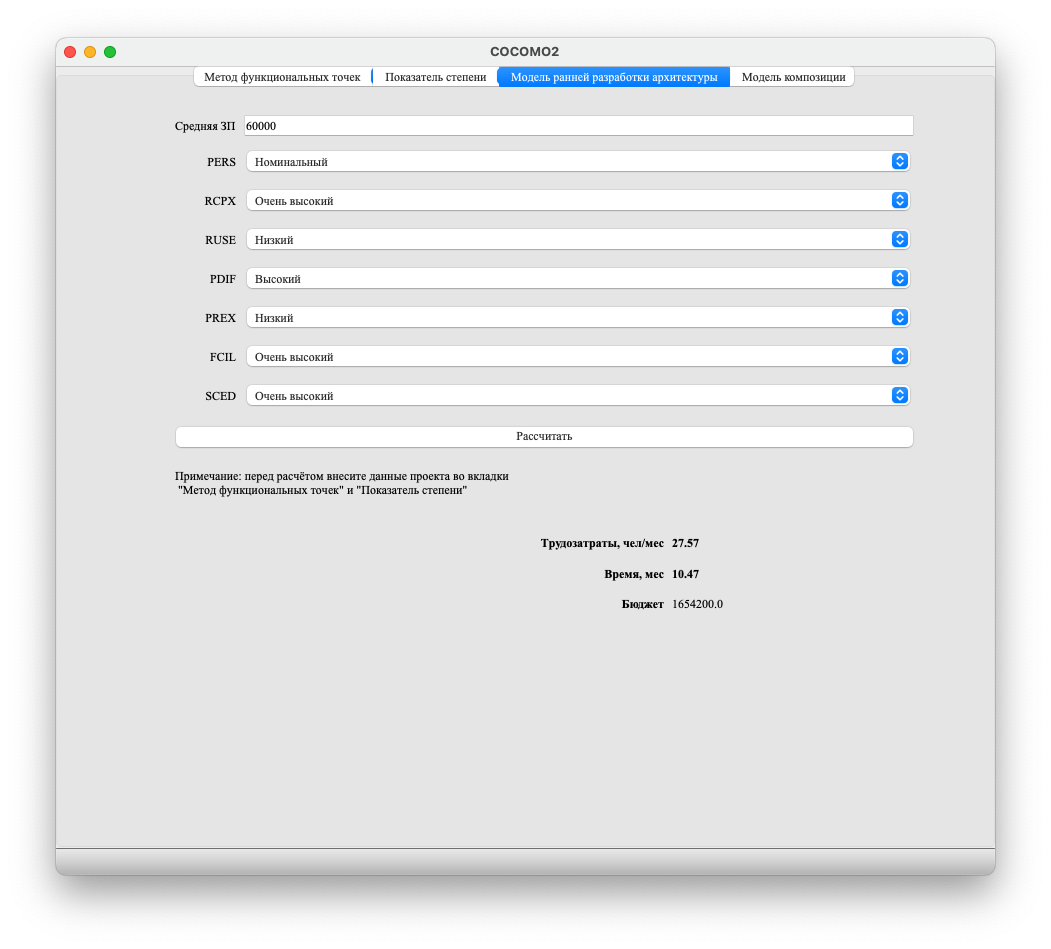
\includegraphics[width=1\linewidth]{assets/images/2.3.png}
	\label{fig:r2}
	\caption{Модель ранней разработки архитектуры}
\end{figure}
\FloatBarrier



\subsection*{Вывод}

В ходе выполнения данной работы была освоена методология оценки параметров проекта COCOMO2 и разработан программный инструмент для её применения. Выполнен анализ выданного задания:
\begin{itemize}
	\item рассчитаны функциональные точки и показатель степени модели (p)
	\item были определены факторы, влияющие на показатель степени
	\item ранней разработки архитектуры приложения
	\item композиции приложения
\end{itemize}

По модели композиции приложения прогноз более благоприятный, чем в модели ранней архитектуры приложения.
Методология COCOMO2 является более сложной по сравнению с COCOMO, но позволяет более тонко настраивать параметры плана, что даёт более точный и детальный прогноз.
